\section{Data and Descriptive Analysis}
\label{sec:descriptive}

This section fixes the object of study and the measuring instrument. We first
describe the panel, the target, and the exogenous information set
(Section~\ref{sec:desc_dataset}); then the causal preprocessing and feature
construction that turn raw series into a design matrix
(Section~\ref{sec:desc_preprocessing}); then the descriptive facts that motivate
the paper's organising claim --- that the predictable component of 30-minute
realized variance is \emph{dense but weak} (Section~\ref{sec:desc_descriptives}).
Section~\ref{sec:desc_protocol} states the evaluation protocol --- walk-forward
design, inverse transform, QLIKE, and the significance machinery --- which every
later section uses without restatement.

\subsection{Dataset and target}
\label{sec:desc_dataset}

The raw data are 30-minute bars for the S\&P 500 complex, gridded to a regular
30-minute frequency and spanning January 2005 through April 2024. The full
regular grid, after the non-trading filter described below, contains
$246{,}057$ rows running from 2005-01-02 19:00 to 2024-04-30 23:00.
% Source: notebooks/features/extractors/spectral_embedding.ipynb (executed output, cell 3)
Because the panel is built on a 24-hour clock covering pre-market, regular, and
after-hours sessions, each 24-hour day contributes $48$ bars: roughly $34$
overnight or extended-session bars and roughly $14$ regular-session bars.
% Source: writeup/session_notes_2026-06-23_feature_investigation.md ("Grid is ~24h: 48 bars/day, ~34 overnight + ~14 RTH")
This is an important and easily missed feature of the design: the majority of
bars are \emph{not} regular-session bars, so any statement about ``intraday''
structure in this panel is a statement about a 24-hour cycle, not about the
$09{:}30$--$16{:}00$ window alone.

Periods in which no venue is open are removed by a fixed calendar filter
implemented in \texttt{src/data/loading.py}: all bars on Friday after
$20{:}00$, all of Saturday, and all of Sunday before $18{:}30$ are dropped. No
other calendar exclusions are applied; holidays and half-days remain in the
panel and are handled by the forward-fill and availability machinery of
Section~\ref{sec:desc_preprocessing} rather than by deletion.

The forecasting target is realized variance measured within each 30-minute bar
as the sum of squared 5-minute log returns, the column \texttt{sumret2} in the
source parquet files:
\begin{equation}
    RV_{d,j} = \sum_{i=1}^{M} r_{d,j,i}^{2}, \qquad M = 6,
    \label{eq:desc_rv}
\end{equation}
where $r_{d,j,i}$ is the $i$-th 5-minute log return inside the $j$-th 30-minute
bar of day $d$. We index bars sequentially as $RV_t$ and forecast one bar ahead,
$RV_{t+1}$. This is the standard realized-measure construction of
\citet{AndersenBollerslevDieboldLabys2003}, sampled at the intraday frequency
for which the heterogeneous autoregressive model of \citet{Corsi2009} was
designed, but pushed one rung finer: the HAR literature's canonical unit is the
trading day, whereas here both the target and the lag ladder live at 30-minute
resolution.

\paragraph{The evaluation panel.}
Feature construction consumes a burn-in of $3{,}125$ bars, the length of the
longest HAR lag, which reduces the usable panel to $242{,}934$ bars.
% Source: writeup/intraday_regime_findings_2026-06-26.md Sec. 10 (cached rank-matrix, 242,934 rows, 48 bars/trading-day)
The walk-forward protocol of Section~\ref{sec:desc_protocol} then consumes a
further $24{,}000$ bars as the initial training window, leaving
\begin{equation}
    n = 218{,}934 \quad \text{evaluated bars,}
    \label{eq:desc_n}
\end{equation}
which is the out-of-sample panel used by \emph{every} table in this paper.
% Source: writeup/incumbent_metrics.json ("n": 218934) and writeup/causal_tune_plus_spectral_standalone.tex (caption)
The backtest is tiled into $100$ contiguous chunks executed in parallel; each
chunk is replayed with a $24{,}000$-bar warm-up halo immediately preceding its
own slice, so that a chunk's first prediction sees exactly the training window it
would have seen in a single uninterrupted pass. Pooling the chunks bar by bar
therefore reproduces the whole-series run exactly rather than approximately.
This matters for the significance tests: because every model arm in the paper is
scored on the same $218{,}934$-row index, all comparisons are bar-for-bar
paired comparisons.

\paragraph{Exogenous information.}
Beyond the target's own history we use $41$ exogenous columns, organised into
eight thematic buckets plus a target-only baseline. The buckets are defined
programmatically in the \texttt{SUBGROUPS} dictionary of
\texttt{src/data/loading.py} by predicates over column names, and they partition
the $41$ columns exactly. Table~\ref{tab:desc_buckets} lists them.

% Source: src/data/loading.py (ALL_FEATURES, SUBGROUPS); availability columns from writeup/master_table_doc.tex (tab:filtered_qlike)
\begin{table}[H]
\centering
\caption{Exogenous feature buckets. Membership is generated by the
\texttt{SUBGROUPS} predicates in \texttt{src/data/loading.py} and partitions the
$41$ exogenous columns exactly ($7+12+6+6+3+3+4 = 41$). ``$n$ present'' is the
number of bars on which the bucket's columns carry an observed (non-imputed)
value; the corresponding fraction is as reported in the source table, whose
tree-panel denominator is approximately $214{,}900$ bars. Buckets not listed with
a count are observed on essentially the full panel.}
\label{tab:desc_buckets}
\begin{tabular}{llrp{4.6cm}rr}
\toprule
Bucket & Members & \# & Example columns & $n$ present & Frac. \\
\midrule
\texttt{baseline}     & target only & 0  & HAR lags of $\widetilde{RV}$, calendar & --- & --- \\
\texttt{moments}      & own-asset moments & 7  & \texttt{sumret}, \texttt{sumabsret}, \texttt{sumbipow}, \texttt{sumautocov} & 214{,}826 & 100.0\% \\
\texttt{liquidity}    & activity / microstructure & 12 & \texttt{sumvolume}, \texttt{numobs}, \texttt{turnover\_ewstock}, \texttt{effspread\_vwstock} & 214{,}920 & 100.0\% \\
\texttt{market\_ew}   & equal-weighted cross-section & 6  & \texttt{sumret2\_ewstock}, \texttt{sumbipow\_ewstock} & 138{,}357 & 64.4\% \\
\texttt{market\_vw}   & value-weighted cross-section & 6  & \texttt{sumret2\_vwstock}, \texttt{sumabsret\_vwstock} & 138{,}357 & 64.4\% \\
\texttt{sentiment}    & social attention & 3  & \texttt{stocktwits\_attention}, \texttt{stocktwits\_sentiment} & --- & --- \\
\texttt{implied\_vol} & options-implied & 3  & \texttt{vix}, \texttt{vvix}, \texttt{vix3m} & --- & --- \\
\texttt{vol\_demand}  & options order flow & 4  & \texttt{voldemand\_spx\_open\_and\_close}, \texttt{voldemand\_all\_open\_only} & 54{,}062 & 25.2\% \\
\midrule
\texttt{all\_features} & union of the above & 41 & --- & --- & --- \\
\bottomrule
\end{tabular}
\end{table}

Two aspects of Table~\ref{tab:desc_buckets} shape the rest of the paper. First,
the buckets are of very unequal richness: \texttt{liquidity} contributes twelve
columns and \texttt{sentiment} three, so a per-bucket comparison confounds
information content with dimensionality unless it is read per feature
(Section~\ref{sec:marginal} does exactly that). Second, availability is
\emph{structurally} unequal. The equal- and value-weighted cross-sectional
aggregates are observed on $138{,}357$ bars and the options order-flow bucket on
only $54{,}062$; the VIX family does not exist for the earliest part of the
sample at all. Handling this by row deletion would make bucket comparisons
incomparable --- an arm using \texttt{implied\_vol} would be scored on a
different, later, and easier sub-sample than an arm using
\texttt{moments}. Section~\ref{sec:desc_preprocessing} describes the
impute-and-indicate construction that removes this confound.

% PENDING table: summary statistics of raw RV (mean, sd, skewness, kurtosis, quantiles) by session segment --- no such table exists in the repo.
% PENDING figure: autocorrelation function of RV and of adjusted sqrt(RV) out to lag 3125 --- no ACF artifact exists in the repo.

\subsection{Preprocessing and feature construction}
\label{sec:desc_preprocessing}

Every series --- the target and all $41$ exogenous columns --- passes through the
same three-stage, strictly causal pipeline:
\begin{equation}
    \text{Raw} \;\xrightarrow{\ \text{Stage 1}\ }\; \text{diurnal adjustment}
    \;\xrightarrow{\ \text{Stage 2}\ }\; \text{semantic transform}
    \;\xrightarrow{\ \text{Stage 3}\ }\; \text{rolling winsorization}.
    \label{eq:desc_pipeline}
\end{equation}
Causality is enforced at every stage: a quantity dated $t$ uses only
observations strictly before $t$.

\paragraph{Stage 1: diurnal adjustment.}
Intraday volatility has a pronounced and largely deterministic time-of-day
profile. Let $s(t) \in \{1,\dots,48\}$ index the time-of-day slot of bar $t$ and
let $\mathcal{W}_t = \{j : j < t,\ s(j)=s(t)\}$ be the set of the most recent
$W = 20$ observations sharing that slot, with at least $5$ required before the
baseline is considered valid. For non-negative series the baseline is the
same-slot rolling mean,
\begin{equation}
    \bar{RV}_{t\mid s} = \frac{1}{|\mathcal{W}_t|}\sum_{j \in \mathcal{W}_t} RV_j,
    \qquad
    \widetilde{RV}_t = \frac{RV_t}{\bar{RV}_{t\mid s}} ,
    \label{eq:desc_diurnal}
\end{equation}
and for signed series (e.g.\ autocovariance) the same-slot rolling standard
deviation is used in place of the mean. The restriction $j < t$, rather than
$j \le t$, is what makes the adjustment non-anticipative. Warm-up bars, before
five same-slot observations have accumulated, pass through with baseline $1$ and
are consumed by the burn-in, so they never enter the evaluation panel.

\paragraph{Stage 2: semantic transforms.}
Each variable class receives a variance-stabilising map chosen from its
support and tail behaviour rather than fitted: $x \mapsto \sqrt{x}$ for squared-
return and volatility-like measures (including $RV$ itself, bipower variation,
turnover and effective spread), $x \mapsto \mathrm{sign}(x)\sqrt{|x|}$ for
autocovariance, $x \mapsto x^{1/3}$ and $x \mapsto x^{1/4}$ for third and fourth
moments, and $x \mapsto \log x$ for the implied-volatility family. Because the
model is trained on the $\sqrt{\cdot}$ scale of $RV$, mapping forecasts back to
raw variance requires an explicit bias correction, given in
Section~\ref{sec:desc_protocol}.

\paragraph{Stage 3: rolling winsorization.}
After transformation each series is clipped to rolling $5$th and $95$th
percentile bounds estimated on the trailing $W_{\mathrm{clip}} = 240$
observations (about five trading days) ending at $t-1$:
\begin{equation}
    x_t^{w} = \mathrm{clip}\!\left(x_t;\ q^{(t)}_{0.05},\ q^{(t)}_{0.95}\right).
    \label{eq:desc_winsor}
\end{equation}
Winsorization is lossy and therefore is \emph{not} inverted at evaluation time;
only Stages 1 and 2 are.

\paragraph{HAR features.}
The target's own history enters through trailing rolling means of the adjusted
series on a base-5 geometric ladder,
\begin{equation}
    \mathcal{L} = \{1,\ 5,\ 25,\ 125,\ 625,\ 3125\},
    \qquad
    \overline{RV}^{(k)}_t = \frac{1}{k}\sum_{i=0}^{k-1}\widetilde{RV}_{t-1-i},
    \label{eq:desc_har}
\end{equation}
spanning roughly $30$ minutes, $2.5$ hours, half a trading day, $2.6$ days,
$13$ days and $65$ trading days. The one-bar shift in
Equation~\eqref{eq:desc_har} keeps contemporaneous information out of the
feature. This is the multi-scale device of \citet{Corsi2009} transposed from the
daily/weekly/monthly triple to a six-rung intraday ladder. The identical ladder
is applied to each exogenous column, so every included exogenous variable
contributes $|\mathcal{L}| = 6$ rolling-mean columns; day-of-week and hour-of-day
dummies are appended for all models.

\paragraph{Missingness: impute-and-indicate.}
Rather than deleting rows with unobserved exogenous values --- which would give
each bucket its own sub-sample and destroy cross-bucket comparability --- each
exogenous column is forward-filled within its availability window, filled with
an in-distribution neutral value where it is structurally absent, and
accompanied by a binary availability indicator column. The linear coefficient on
the indicator absorbs any level shift between the pre- and post-availability
eras, and the value column contributes only where it exists. The result is that
every bucket, including \texttt{implied\_vol} and \texttt{vol\_demand}, lives on
the same $218{,}934$-row index. This is precisely what licenses the bar-for-bar
loss comparisons and the paired significance tests of
Section~\ref{sec:desc_protocol}.

\subsection{Descriptive analysis}
\label{sec:desc_descriptives}

We now report the descriptive facts that the modelling sections take as given.
They fall into three groups: how persistent the target is, what intraday
structure survives the diurnal adjustment, and what the design matrix looks like
geometrically.

\subsubsection{Persistence dominates}

Thirty-minute realized variance is extraordinarily persistent, to the point that
persistence alone is a strong competitor. In a prototype walk-forward exercise
over $4{,}127$ test days --- refitting every five days, on the adjusted target
--- a pure persistence forecast attains mean squared error $0.076277$, an
$R^2$ of $+0.2902$ against a moving-average baseline whose own MSE is
$0.107461$. Both a direct $k$-nearest-neighbour forecast on the six HAR features
(MSE $0.087887$) and a spectral-embedding variant of it (MSE $0.089581$) score
\emph{worse} than simply carrying the last value forward.
% Source: notebooks/features/extractors/spectral_embedding.ipynb (executed output, cell 19)
The lesson is not that nearest neighbours are a bad estimator but that the
conditional mean of $RV_{t+1}$ is overwhelmingly explained by its own recent
level, and that a method which spends its capacity on the \emph{shape} of the
recent path rather than its \emph{level} pays for it. The HAR ladder is the
device that makes level information available at several horizons at once, and
it is a genuinely hard benchmark: a flexible learner given the same six columns
does not automatically improve on it.

The HAR features themselves are exactly what they claim to be. Direct
verification confirms that \texttt{har\_ma\_W} equals the trailing rolling mean
of $RV$ with window $W$ to machine precision, with maximum absolute deviation of
order $10^{-16}$ for $W = 5,\dots,3125$; an exponentially weighted alternative
with matched span correlates only $0.78$--$0.98$ with the realized construction
and is therefore a different feature, not a reparameterisation.
% Source: writeup/OVERNIGHT_RESULTS_2026-06-30.md (HAR construction verification)

\subsubsection{Diurnal structure and what leaks through it}

The Stage-1 adjustment does most, but not all, of the seasonal work. Measured
against the target, the same-slot rolling-mean adjustment removes $77\%$ of the
diurnal variance; the residual $23\%$ leak retains about $48\%$ of the original
diurnal \emph{amplitude} but accounts for only about $4\%$ of total residual
noise.
% Source: writeup/intraday_regime_findings_2026-06-26.md Sec. 6
Driving that leak to zero is therefore not where the remaining predictability
lies, and we do not pursue it.

What does survive, and matters, is not a leftover level pattern but a
\emph{sign change in persistence at session transitions}. Correlating the
five-bar HAR feature \texttt{har\_ma\_5} with the forecast residual and
stratifying by hour of day gives a stable positive association of $+0.05$ to
$+0.13$ through the continuous session, but a negative association at the two
auction boundaries: $-0.085$ at hour $9$, the $09{:}30$ open, and
$-0.085$, $-0.21$, $-0.14$, $-0.03$ across hours $16$ to $19$, the close and the
after-hours window, peaking at $-0.21$ at hour $17$.
Table~\ref{tab:desc_hourcorr} collects these values.

% Source: writeup/intraday_regime_findings_2026-06-26.md Sec. 7 (Test 2, localization by hour)
\begin{table}[H]
\centering
\caption{Correlation of \texttt{har\_ma\_5} with the forecast residual by hour of
day. Positive values indicate the usual volatility-persistence relation;
negative values indicate that the relation \emph{reverses}. The reversal is
sharp and localised at the open and at the close/after-hours window, not gradual
across the session.}
\label{tab:desc_hourcorr}
\begin{tabular}{lr}
\toprule
Hour of day & $\mathrm{corr}(\texttt{har\_ma\_5},\ \text{residual})$ \\
\midrule
Continuous session (typical) & $+0.05$ to $+0.13$ \\
$9$ (open, $09{:}30$)        & $-0.085$ \\
$16$ (close)                 & $-0.085$ \\
$17$                         & $-0.21$ \\
$18$                         & $-0.14$ \\
$19$                         & $-0.03$ \\
\bottomrule
\end{tabular}
\end{table}

Two properties of this reversal are worth recording here because
Section~\ref{sec:linvsnonlin} depends on them. It is \emph{clock-anchored} and
not volatility-state-anchored: interacting the HAR features with clock regimes
adds $+0.0095$ out-of-sample $R^2$ on the residual, of which $+0.0079$ survives
without any hour main effect, whereas interacting them with a
volatility-state regime built from $RV$ relative to its diurnal norm \emph{loses}
$-0.0027$.
% Source: writeup/intraday_regime_findings_2026-06-26.md Sec. 6 (honest OOS test)
And it is sharp rather than smooth --- it appears at the boundaries and not in
the last slot of the session --- which is the signature of an
auction/session-transition mechanism rather than a mis-specified seasonal curve.
A structure of this kind is invisible to a linear model in the HAR coordinates
but is exactly the kind of thing a tree can split on, which is why the
linear-versus-nonlinear question of Section~\ref{sec:linvsnonlin} is a question
about \emph{interactions with the clock} rather than about curvature in the
volatility level.

% PENDING figure: mean level of raw RV by time-of-day slot (the diurnal profile itself), before and after Stage-1 adjustment --- no such figure exists in the repo.

\subsubsection{Design-matrix geometry: dense but weak}

The full \texttt{all\_features} design matrix has $p = 529$ columns, decomposing
into $6$ HAR columns, $270$ availability indicators, and $253$ exogenous value
columns --- that is, slightly more than half the matrix encodes \emph{whether} a
series was observed rather than what it said. Table~\ref{tab:desc_geometry}
summarises its geometry.

% Source: writeup/intraday_regime_findings_2026-06-26.md Sec. 2--3
\begin{table}[H]
\centering
\caption{Geometry of the full \texttt{all\_features} design matrix on the
evaluation panel. The participation ratio is the effective number of directions
carrying covariance mass; the numerical rank counts non-degenerate directions.}
\label{tab:desc_geometry}
\begin{tabular}{lr}
\toprule
Quantity & Value \\
\midrule
Columns $p$                                   & $529$ \\
\quad HAR columns                             & $6$ \\
\quad availability indicators                 & $270$ \\
\quad exogenous value columns                 & $253$ \\
Constant always-on indicators                 & $164$ ($31\%$ of $p$) \\
Aspect ratio $p/N$                            & $\approx 0.0022$ \\
Covariance participation ratio                & $\approx 6.8$ \\
Eigenvalue decay exponent                     & $\approx i^{-3.13}$ \\
Numerical rank                                & $317$ (of $529$) \\
Share of target variance carried by PC1 (variance $48$) & $\approx 0\%$ \\
\bottomrule
\end{tabular}
\end{table}

Read together these numbers describe an unusual and consequential situation.
The problem is emphatically not high-dimensional in the statistical sense: with
$p/N \approx 0.0022$ there are roughly $450$ observations per column, so
classical asymptotics apply and overfitting is not the binding constraint. The
covariance spectrum is steep --- decaying like $i^{-3.13}$, with a participation
ratio near $6.8$, meaning that essentially all the variance in $529$ columns
lives in about seven directions --- and $212$ of the $529$ directions are
numerically degenerate. A third of the matrix ($164$ columns, $31\%$) is
constant: always-on availability flags for series that are never missing, which
carry no information at all and which an $\ell_1$-penalised fit assigns exactly
zero weight in every refit.

The decisive fact, however, is the last row of
Table~\ref{tab:desc_geometry}. The leading principal component, with variance
$48$, carries approximately \emph{none} of the target signal. Unsupervised
compression is therefore misaligned with prediction: the directions that explain
the predictors do not explain the response. The punchline that organises the
remainder of this paper is that \emph{variance concentrates in a few directions
but the signal does not live there}. The predictable component is dense in the
original coordinate basis --- spread thinly across many columns, each
contributing a little --- and weak in every direction, including the
high-variance ones. That combination rules out the two standard shortcuts at
once: dimension reduction discards signal because signal is not aligned with
variance, and aggressive sparsity discards signal because no small set of
columns carries it. It is the regime in which the marginal-contribution analysis
of Section~\ref{sec:marginal}, the linear-versus-nonlinear comparison of
Section~\ref{sec:linvsnonlin}, and the algorithmic choices of
Section~\ref{sec:algorithms} all have to operate.

\subsubsection{Behaviour in crisis windows}

Finally, it is worth seeing what the baseline actually does when volatility
moves. Figures~\ref{fig:desc_crash2008} and~\ref{fig:desc_crash2020} plot the
HAR baseline's forecast against realized $RV$ through the two most violent
episodes in the sample: the September--November 2008 Lehman/TARP window and the
February--April 2020 COVID window. The forecast tracks the level regime
faithfully but systematically undershoots the peak bars --- the visual
counterpart of a Mincer--Zarnowitz slope below one
(Section~\ref{sec:desc_protocol}), and a reminder that QLIKE, which penalises
under-prediction asymmetrically, is the right loss for this target.

% Source: writeup/figures/crash_2008_ridge.png (canonical source results/diagnostics/ridge_har_paper/crash_2008.png)
\begin{figure}[H]
\centering
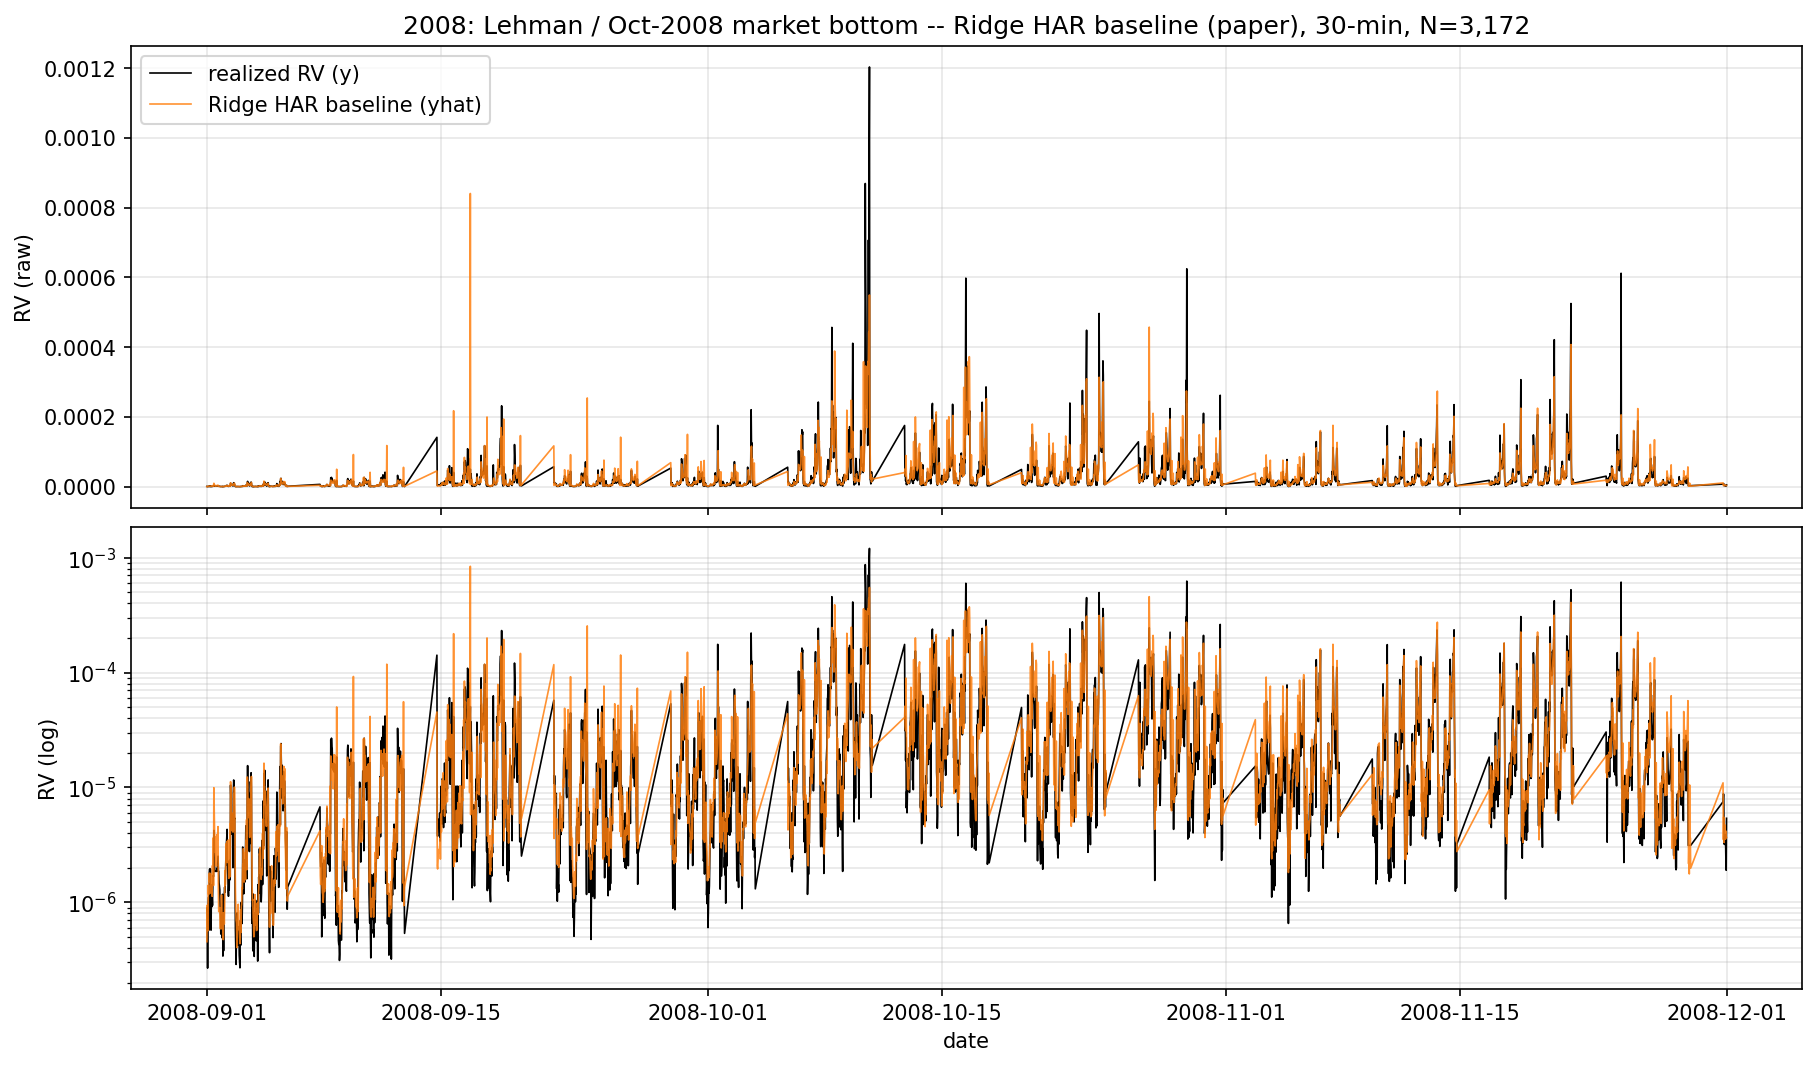
\includegraphics[width=\linewidth]{figures/crash_2008_ridge.png}
\caption{HAR baseline forecast versus realized $RV$, 30-minute bars,
2008-09-01 through 2008-11-30 (Lehman collapse 2008-09-15; TARP; the
October 10 equity-market bottom). Linear and logarithmic scales.}
\label{fig:desc_crash2008}
\end{figure}

% Source: writeup/figures/crash_2020_ridge.png (canonical source results/diagnostics/ridge_har_paper/crash_2020.png)
\begin{figure}[H]
\centering
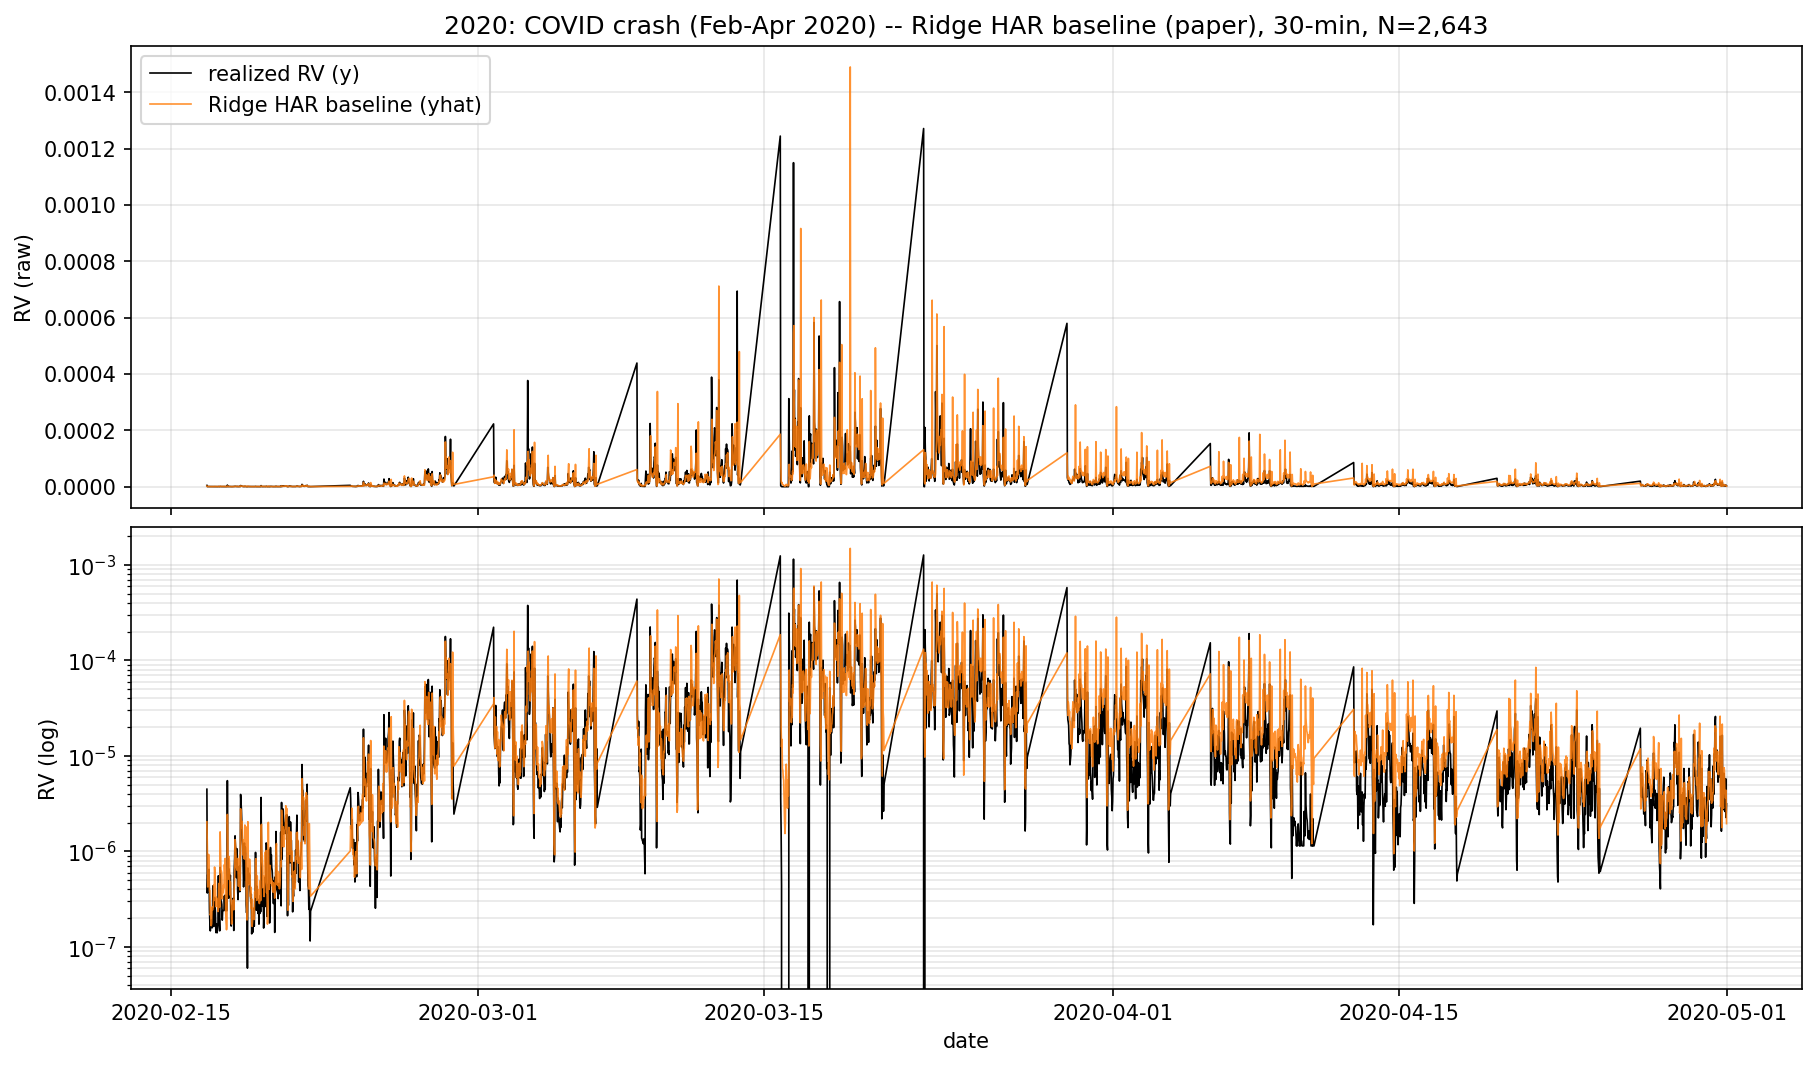
\includegraphics[width=\linewidth]{figures/crash_2020_ridge.png}
\caption{HAR baseline forecast versus realized $RV$, 30-minute bars,
2020-02-15 through 2020-04-30, with the COVID volatility peak around the
March 16 session. Linear and logarithmic scales.}
\label{fig:desc_crash2020}
\end{figure}

\subsection{Evaluation protocol}
\label{sec:desc_protocol}

All results reported in Sections~\ref{sec:marginal}--\ref{sec:algorithms} follow
the protocol stated here.

\paragraph{Walk-forward design.}
Forecasts are produced by a strictly causal rolling-origin procedure. At bar $t$
the model may use only data dated strictly before $t$. The training window is
the immediately preceding $500$ trading days, or $24{,}000$ bars at $48$ bars per
day; one prediction is produced per bar; the window then slides by one bar.
Linear models are refit at \emph{every} bar --- not every $k$ bars --- which is
computationally feasible only because the sliding-window normal equations admit
exact rank-1 up/down-dating, the estimator machinery described in
Section~\ref{sec:algorithms}. The backtest is tiled into $100$ contiguous
chunks, each replayed with its own $24{,}000$-bar warm-up halo, and the per-bar
predictions are pooled; as noted above this reproduces a single uninterrupted
pass exactly.

\paragraph{Inverse transform and smearing correction.}
Models are estimated on the adjusted, square-root scale, but evaluation is on
raw variance. Since $\mathbb{E}[\sqrt{X}]^2 \neq \mathbb{E}[X]$, naively squaring
a forecast of $\sqrt{RV}$ is downward biased. We apply Duan's smearing estimator
\citep{Duan1983}, adding the in-sample residual variance before inverting Stage
2 and then undoing the Stage-1 diurnal division:
\begin{equation}
    \widehat{RV}^{\mathrm{raw}}_t
    = \left(\hat{f}_t^{\,2} + \hat{\sigma}^2_{\varepsilon}\right)\cdot
      \bar{RV}^{\mathrm{baseline}}_{t\mid s},
    \qquad
    \hat{\sigma}^2_{\varepsilon} = \frac{1}{N}\sum_i (y_i - \hat{y}_i)^2,
    \label{eq:desc_duan}
\end{equation}
where $\hat{f}_t$ is the forecast on the adjusted square-root scale and
$\bar{RV}^{\mathrm{baseline}}_{t\mid s}$ is the diurnal baseline of
Equation~\eqref{eq:desc_diurnal}. Stage 3 (winsorization) is lossy and is not
inverted.

\paragraph{Primary loss.}
The primary metric is QLIKE on the raw variance scale, the loss function that is
robust to noise in the volatility proxy \citep{Patton2011}:
\begin{equation}
    L_{\mathrm{QLIKE}}
    = \frac{1}{N}\sum_{t=1}^{N}\left[\, r_t - \log r_t - 1 \,\right],
    \qquad
    r_t = \frac{RV^{\mathrm{raw}}_t}{\widehat{RV}^{\mathrm{raw}}_t}.
    \label{eq:desc_qlike}
\end{equation}
QLIKE is scale-invariant in the level of volatility and penalises
under-prediction far more heavily than over-prediction, which is both the
economically relevant asymmetry and, given the crisis-window behaviour of
Figures~\ref{fig:desc_crash2008}--\ref{fig:desc_crash2020}, the discriminating
one. Secondary metrics are mean squared error and mean absolute error, an
out-of-sample $R^2$ measured against a stated reference forecast,
\begin{equation}
    R^2_{\mathrm{OOS}} = 1 - \frac{\mathrm{MSE}_{\mathrm{model}}}
                                  {\mathrm{MSE}_{\mathrm{reference}}},
    \label{eq:desc_oosr2}
\end{equation}
and the Mincer--Zarnowitz regression of the realization on the forecast
\citep{MincerZarnowitz1969}, whose intercept $\alpha$ and slope $\beta$ diagnose
unconditional bias and forecast over-reactiveness respectively.

\paragraph{The incumbent.}
Every table in this paper is referenced to a single fixed comparator, which we
call \emph{the incumbent}: ordinary least squares on the HAR ladder plus
calendar dummies, with no exogenous features, refit at every bar. It is obtained
from the production ridge path at $\alpha = 0$, hence exact OLS.
Table~\ref{tab:desc_incumbent} states its scores on the evaluation panel.

% Source: writeup/incumbent_metrics.json
\begin{table}[H]
\centering
\caption{The incumbent benchmark: OLS on HAR $+$ calendar features, no exogenous
variables, per-bar refit, scored on the diurnally adjusted panel. QLIKE is on
raw variance after the smearing correction of
Equation~\eqref{eq:desc_duan}; MSE and MAE are on raw variance.}
\label{tab:desc_incumbent}
\begin{tabular}{lr}
\toprule
Metric & Value \\
\midrule
QLIKE                        & $0.13415$ \\
Out-of-sample $R^2$          & $0.694$ \\
Mincer--Zarnowitz $\beta$    & $0.930$ \\
Mincer--Zarnowitz $R^2$      & $0.698$ \\
MSE                          & $4.336\times 10^{-11}$ \\
MAE                          & $1.283\times 10^{-6}$ \\
Bars $n$                     & $218{,}934$ \\
\bottomrule
\end{tabular}
\end{table}

The Mincer--Zarnowitz slope of $0.930$ confirms the visual reading of the crisis
figures: the incumbent is mildly over-reactive, moving more than the realization
does, and so undershoots the largest bars.

\paragraph{Significance.}
Point differences in QLIKE at the fourth decimal place are not self-evidently
meaningful, so every comparison in this paper is accompanied by a test. We use
the Diebold--Mariano test on the per-bar QLIKE loss differential
\citep{DieboldMariano1995}, with a Newey--West heteroskedasticity- and
autocorrelation-consistent long-run variance --- necessary because loss
differentials at 30-minute frequency are strongly autocorrelated --- and the
small-sample correction of \citet{HarveyLeybourneNewbold1997}. Negative
$t$-statistics favour the arm over the comparator. Where several arms are
compared simultaneously we report the Model Confidence Set of
\citet{HansenLundeNason2011} at the stated confidence level, which returns the
subset of models that cannot be distinguished from the best at that level rather
than a single spurious winner. Because impute-and-indicate puts every arm on the
identical $218{,}934$-row index, all these tests are exact paired bar-for-bar
comparisons; no alignment or re-indexing is required, and no arm is advantaged by
being scored on an easier sub-sample. This design follows the emphasis on
honest, protocol-level comparison in the machine-learning-for-asset-pricing
literature \citep{gu2020empirical, christensen2023machine}.

\paragraph{A warning on QLIKE levels across panels.}
QLIKE is scale-free in volatility but \emph{not} comparable across different
preprocessing choices, and the research record behind this paper contains three
mutually incompatible level regimes. First, the diurnally adjusted panel used
throughout this paper, on which competitive arms score in the range
$0.126$--$0.134$ and the incumbent scores $0.13415$. Second, a COVID-inclusive
every-bar battery run on a different evaluation window, on which the same class
of models scores in the range $0.142$--$0.149$.
% Source: writeup/SESSION_HANDOFF_2026-07-02.md (Table 1 HAR QLIKE 0.149) and writeup/OVERNIGHT_RESULTS_2026-06-30.md
Third, a raw research panel with \emph{no} diurnal adjustment, on which the same
HAR baseline scores $0.786$ and feature-bundle arms score in the range
$0.35$--$0.79$, because the seasonal channel that Stage 1 removes is still in
the loss and inflates every gain measured against it.
% Source: writeup/SESSION_HANDOFF_2026-07-02.md (raw research panel caveat: HAR QLIKE 0.786 vs 0.149; best combo 0.34598, all-8 0.35156)
A difference of $0.4$ QLIKE units between two tables can therefore reflect
nothing but a preprocessing choice. Every comparison made in this paper stays
strictly within one regime, and every table is labelled with the panel it was
computed on.
